\documentclass[conference]{IEEEtran}
\IEEEoverridecommandlockouts
% The preceding line is only needed to identify funding in the first footnote. If that is unneeded, please comment it out.
\usepackage{cite}
\usepackage{amsmath,amssymb,amsfonts}
\usepackage{algorithmic}
\usepackage{graphicx}
\usepackage{textcomp}
\usepackage{xcolor}
\usepackage{subfigure}
\def\BibTeX{{\rm B\kern-.05em{\sc i\kern-.025em b}\kern-.08em
    T\kern-.1667em\lower.7ex\hbox{E}\kern-.125emX}}
\begin{document}

\title {Combining Fine-grained Font Recognition and OCR for Reading Historical Documents}

\author{\IEEEauthorblockN{Souptik Sen}
\IEEEauthorblockA{\textit{Friedrich-Alexander-Universität Erlangen-Nürnberg} \\
Erlangen, Germany\\
souptik.sen@fau.de}
}

\maketitle

\begin{abstract}
Handwritten text analysis is a widely employed methodology in the domain of machine learning, and has proven to be highly effective in delivering notable success on specific tasks. The goal of this project is to investigate a novel approach to combine fine-grained font recognition with OCR for books printed from the 15th to the 18th century. We have used a dataset of OCR for early printed books for which font groups of each character have been manually labeled. Books from this era frequently include font group changes that occur in the middle of lines or even words, indicating linguistic shifts. We examine eight distinct font groups found in our collection of samples. In this study, we have utilized an Entity transformer model to perform OCR (Optical Character Recognition) and simultaneously assign font groups to the predicted characters from our dataset of historical documents. The results demonstrate that this approach is effective in performing OCR  alongside fine-grained font recognition of multiple font groups from historical images simultaneously. However, the text prediction performance of this approach is not satisfactory, therefore in the future, we will need to improve the text classification quality.
\end{abstract}

\section{Introduction}
Massive volumes of meticulously scanned documents of various kinds are being published by libraries and archives. This creates the need for effective techniques to handle the volume of data. In many circumstances, researchers can benefit greatly from having the document content as a text file rather than an image file since it makes it easier for them to search for specific information. However, digitizing older means of documentation constitutes a more challenging task and requires significantly more effort. The main goal of this work is to combine fine-grained font group classification and OCR of early modern prints - documents printed between the 15th and the 18th centuries.\newline
To achieve this, section \ref{data} covers the data analysis and required preparation steps to make the data usable for our Entity transformer model. The semantic and visual features are extracted from the early modern print images using a deep learning-based neural network architecture and converted to a representation more suitable for our model translation. This will be explained in the section \ref{visual_feat}. Likewise, the features of the text and font information are also converted into machine-interpretable representations separately and fused, which will be explained in detail in section  \ref{sem_feat}. The visual features are then refined inside our transformer encoder module, and finally, the refined visual information is fused with the combined text and font information flow in our transformer decoder module. This is described in more depth in the section \ref{combinded_feat}. After this, the output from the transformer decoder module is split and each extracted split is passed through a separate deep learning-based classification layer to get our text and font prediction, which will also be explained in section \ref{combinded_feat}. This work continues with the evaluation subsection \ref{evaluation} following a summary of training settings and hyper-parameters in section \ref{training}. In section \ref{evaluation} we investigate how our model performs on completely unseen test images based on several metrics. Subsequently, the paper concludes with section \ref{discussion} providing a summary of the findings and section \ref{conclusion} offering a tentative outlook.


\section{Dataset analysis and preprocessing}\label{data}
An overview of the data used and how they are made available for our model is provided in this section.

\subsection{Dataset analysis}
We used 2,506 pages from 849 books published between the 15th and the 18th centuries to compile our data. Our data has been split at the book level so that no data from the same book can be present in both training and test sets. We have considered eight distinct font groups which is a subset of two super font groups, namely Gothic and Roman. The font groups that compose the Gothic font groups are Bastarda, Fraktur, Rotunda, Schwabacher, and Textura. The font groups constituting the Latin font groups are Italic and Antiqua. We have also used Gotico-Antiqua, which falls halfway between Goth and Roman Latin fonts. Along with the mentioned font groups, we have also added extra groups to signify padding and the end of a sequence which will be explained in more detail in this section. Our dataset is constructed by splitting the pages of the books into small individual text lines like in \cite{faucris.312972480}, an example of which can be found in Fig. \ref{example}.\newline
\begin{figure}[htbp]
    \centering
    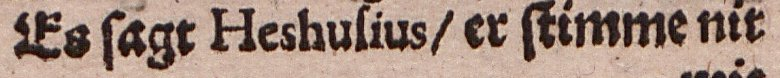
\includegraphics[width=0.5\textwidth]{figures/Example_Line_image.jpg}
    \caption{Example line image}
    \label{example}
\end{figure}\newline
To compile our dataset we have used these individual text line images, which contain on average about 20 characters, along with information like text documents that include the contained ground truth text in the corresponding text line image and also pickled NumPy arrays that comprised the ground truth font group labels for individual characters in the corresponding text line image. The ground truth text string corresponding to our example line image in Fig \ref{example} can be found in Fig.\ref{GT}. 
\begin{figure}[htbp]
    \centering
    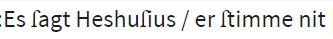
\includegraphics[width=0.5\textwidth]{figures/GTText.png}
    \caption{Ground Truth Text String of Example Line Image}
    \label{GT}
\end{figure}\newline
All the letters that appear in the dataset, combined with extra padding, end of sequence, and start of sequence tokens, are used to create the alphabet dictionary used for character tokenization. This allows the use of the Smooth Cross Entropy loss, which is further discussed in section \ref{training}.
\subsection{Dataset preprocessing}

\begin{table}[htbp]
\caption{Overview random data augmentation for semantic features}
\begin{center}
\begin{tabular}{|c|c|}
\hline
\textbf{\textit{Method}} & \textbf{\textit{Probability}}  \\
\hline
Elastic distortion \cite{yousef2020origaminet} & 0.6 \\
\hline
Random transformes \cite{yousef2020origaminet} & 0.6 \\
\hline
Dilation \& Erosion & 0.6 \\
\hline
Contrast adjustment & 0.6 \\
\hline
Random perspective \cite{NEURIPS2019_9015} & 0.6 \\
\hline
\end{tabular}
\label{data_aug}
\end{center}
\end{table}
The individual text line images are augmented using several random augmentation techniques, binarized, and resized to a fixed height and width of 256 pixels to make the data usable for our model architecture. Binarization has been applied by utilizing the sauvola thresholding proposed in \cite{SAUVOLA2000225}. Table \ref{data_aug} contains the random augmentation techniques that have been used on our images. The final processed and augmented version of our example image i.e. Fig.\ref{example} can be seen in Fig. \ref{line_img}. \newline
\begin{figure}[htbp]
    \centering
    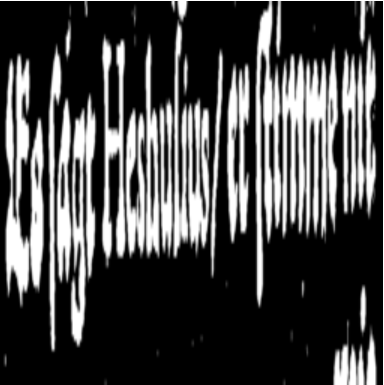
\includegraphics[width=0.3\textwidth]{figures/processed_line_image.png}
    \caption{Fully processed Example line image}
    \label{line_img}
\end{figure}\newline
The augmented and processed line images are then provided with the ground truth text and font class information. These individual line information are then stacked together into batches of data. Since we are dealing with a sequence of images, sequence padding is applied to the images to ensure uniform length along the sequence or temporal dimension, assisting efficient batch processing in our model. For the ground truth text documents, each character of the text lines is tokenized by mapping them to their corresponding positions in the alphabet dictionary constructed by us. We also add the 'start of sequence' and the 'end of sequence tokens' to each tokenized text line for our machine to comprehend each text sequence separately. Similarly, we also tokenize the font sequences by mapping each font class to a separate token signifying that particular font group. Every tokenized font sequence additionally has an "end of sequence" token added to it. For every tokenized font sequence, we use the same token to signify the 'start of sequence' and padding.  Due to shape dependencies of our Handwritten Text Recognition model, the batches of ground truth text and font sequences have to be padded to a fixed sequence length matching the longest corresponding sequence for each batch. This is done by adding extra padding tokens after 'end of sequence' tokens for the tokenized batches of text and font sequences.\newline
The test set was created using random combinations of font groups with at least 10,000 characters, minimizing the variance of the number of characters per font group. Similar methods were used to obtain the validation set, albeit with less data. All metrics presented in section \ref{evaluation} are based on the aforementioned test set. It is important to note that we have used both single-font line images and multiple-font line images collectively for training and validating our model.

\section{Methods}
The architecture of the model utilized will be covered in more detail in this section. We have used an entity transformer model based on \cite{rouhoua2021transformerbased} to jointly perform Handwritten Text Recognition and fine-grained font recognition for the recognized characters. This is done by concatenating the entity tags of our alphabet tokens with the entity tags of our font class tokens, therefore visualizing them as different entity tags for the same input sequence, thus making them a part of the output sequence to predict. The architecture of our model is depicted in Fig. \ref{htr_arch}.
\begin{figure*}[htbp]
    \centering
    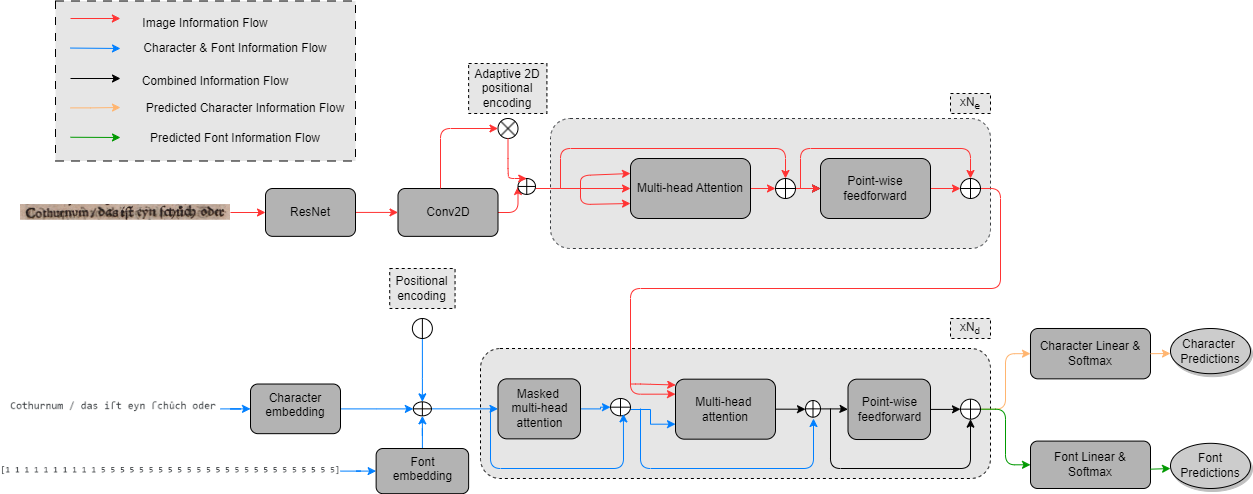
\includegraphics[width=1.0\textwidth]{figures/HTRModelArchitecture.png}
    \caption{Architecture of the transformer HTR model}
    \label{htr_arch}
\end{figure*}
\subsection{Visual Feature Extraction}\label{visual_feat}
Firstly the line image is fed into a pre-trained ResNet-18 model \cite{7780459} for extracting the visual features. This reduces the high computational cost of the self-attention layers inside the encoder module of the entity transformer, putting more emphasis on the sequence part as mentioned in \cite{faucris.276690551}. To make the 2-dimensional feature maps accessible by the transformer encoder, the next step is to squeeze them into a sequence that matches the encoder input dimension. This is done by applying a 2D Convolutional layer on the feature map output of the ResNet-18 model. Before reshaping the feature maps to a sequence, a positional encoding must be added to them, due to the positional invariance of the self-attention layers. Our dataset consists of highly cursive writing. We have employed the adaptive 2D positional encoding mentioned in \cite{lee2019recognizing} to the extracted feature maps to be more robust to highly cursive writing.
Based on the feature map and learned weights, a scaling parameter will be computed for each spatial dimension (\(\alpha\), \(\beta\)). The positional encoding is then added to the feature map \(F\) using these values:
\begin{equation}\label{AD2DPE}
\tilde{F}_{\tilde{h},\tilde{w}} = {{F_{h,w} + \left( \alpha(F)P^{\sin u}_{h} + \beta(F)P^{\sin u}_{w} \right),}} \tag{1}
\end{equation}
where \(P^{\sin u}\) is defined as \( P^{\sin u}_{p, 2i} = \sin\left(\frac{p}{{10000}^{2i/D}}\right) \) and \( P^{\sin u}_{p, 2i+1} = \cos\left(\frac{p}{{10000}^{2i/D}}\right) \). Here \( p \) and \( i \) are the indices of the position and the hidden dimension, and \( D \) is the size of the hidden dimension.\newline

\subsection{Character and Font fusion}\label{sem_feat}

The target sequence utilized in our model architecture is comprised of the character and font sequences. The character logits and the font logits bear positional dependency with each other, i.e. for every character logit, there is a corresponding font logit. To preserve the positional interdependency of the character and font sequences, it is crucial that we carefully consider how to concatenate them for the machine to interpret. The positional interdependence is destroyed if the concatenated sequence is flattened to fit the decoder input dimension. Thus we come up with a different approach to fuse the character and font information. Two separate embedding layers have been used, one for character embedding and another for font embedding. The target character logits are embedded into a higher dimensional space by using the character embedder. Similarly, the font class logits from the target sequence are also embedded into a higher dimensional space by the font embedding layer. Our model's total embedding dimensions,  \(T\), are divided into two  \(T/2\) dimensional embedding spaces, one for character embedding and one for font embedding. Ultimately, after positional encoding, these embeddings are concatenated along our target sequence's last axis, resulting in character embeddings for the first  \(T/2\) dimensions and font embeddings for the next  \(T/2\) dimensions. A visual illustration can be seen in Fig. \ref{cf}.

\begin{figure}[htbp]
    \centering
    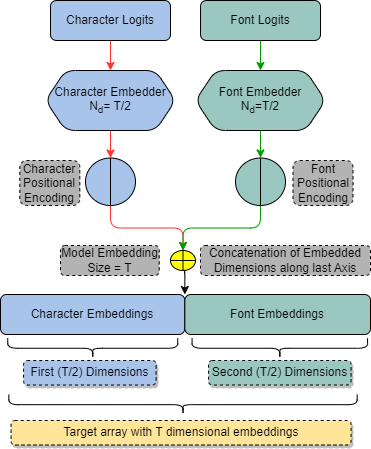
\includegraphics[width=0.4\textwidth]{figures/Character&Font .png}
    \caption{Character and Font Fusion}
    \label{cf}
\end{figure}

Again, due to the positional invariance of the self-attention layers in the decoder module, we have to add sinusoidal positional encoding \cite{vaswani2017attention} to the two \(T/2\) embeddings separately before concatenating them. The sinusoidal positional encoding applied can be represented by the following equations:
\begin{equation}\label{1D_pos_1}
{PE}_{(p, 2i)} = \sin\left(\frac{{p}}{{10000}^{\frac{2i}{d}}}\right), \tag{2}
\end{equation}

\begin{equation}\label{1D_pos_2}
{PE}_{(p, 2i + 1)} = \cos\left(\frac{{p}}{{10000}^{\frac{2i}{d}}}\right), \tag{3}
\end{equation}
Here, the location of the token in the sequence is denoted by \(p\), the dimension by  \(i\), and the dimensionality of the positional encoding by  \(d\). For our model, the dimensionality of the positional encoders can be expressed by \(d = d_{font} = d_{char} = T/2\)  .\newline

\begin{equation}\label{pos_encoding_addition_character}
\tilde{C}_{(p_c)} = T_c + \sum_{i_c=0}^{d-1} \left( \text{PE}_{(p_c, 2i_c)} + \text{PE}_{(p_c, 2i_c+1)} \right), \tag{4}
\end{equation}

\begin{equation}\label{pos_encoding_addition_font}
\tilde{F}_{(p_f)} = T_f + \sum_{i_f=0}^{d-1} \left( \text{PE}_{(p_f, 2i_f)} + \text{PE}_{(p_f, 2i_f+1)} \right), \tag{5}
\end{equation}

\begin{equation}\label{pos_encoding_addition_font_character}
\tilde{T}_{(p)} = \tilde{C}_{(p_c)} + \tilde{F}_{(p_f)} , \tag{6}
\end{equation}
Here, \(T_c\) and \(T_f\) represent the character and font-embedded vectors respectively. \(\tilde{C}_{(p_c)}\) and \(\tilde{F}_{(p_f)}\) represents the feature vectors after adding the respective positional vector components to the original character embedded vector \(T_c\) and the original font embedded vector \(T_f\) respectively. The final target feature vector, \(\tilde{T}_{(p)}\), is formed by adding the respective feature vectors \(\tilde{C}_{(p_c)}\) and \(\tilde{F}_{(p_f)}\). The final target feature vector will have \(T\) embeddings, after the concatenation of the respective two \(T/2\) character and font embeddings.

In order to shorten the training period, this step can be parallelized by masking the target or decoder's input sequence's unseen segments during training\cite{faucris.276690551}. We refer to this as teacher forcing. It should be noted that during inference, the model predicts the outputs in an auto-regressive manner without the use of teacher forcing. In other words, the model receives the start-of-sequence token for character prediction inference and the padding sequence token for the font classification inference in the first iteration and adds the best fit of each prediction to the sequence until an end-of-sequence token appears. Teacher forcing during training leads to a problem when dealing with lower amounts of data, like historical documents, since the model quickly overfits the input target or decoder sequence without incorporating the visual features in the mutual attention layers. Therefore, during training and validation, we decided to perturb the input sequence of the decoder to make the model more robust to predicted errors and to force the model to rely more on the encoder features\cite{faucris.276690551}.


\subsection{Fusion Of Visual, Text and Font information}\label{combinded_feat}
\subsubsection{Visual Feature Refinement}\label{Visual_refine}
To further condense the visual information the transformer encoder module is applied \(N_e\) times on the flattened output of \(\tilde{F}\). The multi-headed self-attention layer \cite{vaswani2017attention} is employed there; the following equation does not depict the splitting into several heads for simplicity's sake:
\begin{equation}\label{attention}
\hat{F} = \text{Softmax}\left(\frac{QK}{\sqrt{d}}\right) V \tag{7}
\end{equation}
\begin{equation}\label{attention_mechanism}
\quad Q = \tilde{F}W_Q \quad K = \tilde{F}W_K \quad V = \tilde{F}W_V \tag{8}
\end{equation}
In this context, the query (\(Q\)) is determined by the feature map (\(\tilde{F}\)) multiplied by the parameter matrix (\(W_Q\)), the key (\(K\)) is derived from (\(\tilde{F}\)) using the parameter matrix(\(W_K\)), and the value (\(V\)) is computed as (\(\tilde{F}W_V\)) using the parameter matrix  \( W_V \). A point-wise feed-forward layer is
attached to the attention mechanism, which is used for further refinement of \(\hat{F}\). The flow of visual features in the transformer encoder is depicted in figure \ref{encoder}.

\begin{figure}[htbp]
    \centering
    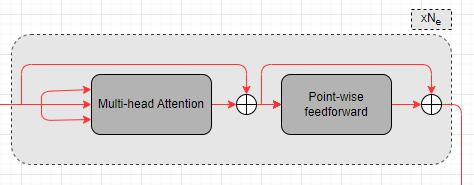
\includegraphics[width=0.5\textwidth]{figures/Encoder.png}
    \caption{Visual Information Flow in Encoder}
    \label{encoder}
\end{figure}

\subsubsection{Character and Font Information Flow in decoder}\label{Character_and_font}
The Transformer Decoder layer will be applied \(N_d\) times on the fused character and font embeddings \(\tilde{T}\). Here, the multi-headed self-attention is applied on \(\tilde{T}\) to condense the context information. Thus, like the final visual vector \(\hat{F}\) we get a vector \(\hat{T}\) by applying the equations \ref{attention} and \ref{attention_mechanism} to  \(\tilde{T}\).
\subsubsection{Fusion}\label{Fusion}
In the following step, inside the Transformer Decoder, the mutual attention layer fuses the visual information \(\hat{F}\) with the textual and font information \(\hat{T}\) by setting 
\begin{equation}\label{second_attention_mechanism}
\quad Q = \hat{T}W_Q \quad K = \hat{F}W_K \quad V = \hat{F}W_V \tag{9}
\end{equation}
and applies the same formula as in the equation \ref{attention}. After running through the transformer decoder multiple times the output sequence having dimensions \(T\) is split along the last axis to get two sequences that have \(T/2\) dimensions in their last axis. The first sequence forms the predicted character sequence, which is then fed to a linear layer to match the alphabet vocabulary size and then finally passed through a softmax layer to get the probability scores of the next character. The second sequence yields the predicted font class sequence, which is then fed to a separate linear layer to match the font class vocabulary size and then ultimately passed through a softmax layer to get the confidence scores of the font class of the next predicted character. Figure \ref{decoder} represents the combined information flow inside the transformer decoder.
\begin{figure}[htbp]
    \centering
    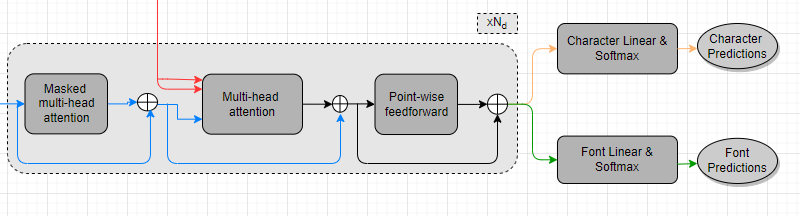
\includegraphics[width=0.5\textwidth]{figures/Decoder.png}
    \caption{Combined Information Flow in Decoder}
    \label{decoder}
\end{figure}
\newpage
\section{Training}\label{training}
We will walk through our model's training procedure in this part. In our work, we have employed two distinct Smooth cross-entropy loss functions: one for font prediction and the other for character prediction. During backpropagation, the model is trained to simultaneously optimize both character prediction and font class prediction by adding these two losses multiplied with their appropriate weights,\(\text{Weight}_\text{char}\) and \(\text{Weight}_\text{font}\), and logging the cumulative total loss for backpropagation. To ensure that the model gives equal importance to both font class prediction and character prediction, we have set both weights for our loss function to a value of $1$. For training our model early stopping has been applied with a patience of $10$, monitoring the validation total loss i.e. the sum of our two Cross Entropy Losses. Batch size has been set to $4$, and a learning rate of $0.0001$ is applied for training. The probability of random character and random font class labels with noisy teacher forcing is $20$\%. The transformer encoder and decoder have a hidden dimension of $256$ with $2$ attention heads and $N_e = N_d = 2$. Dropout is set to $0.1$. For training our model we have used the AdamW optimizer \cite{loshchilov2019decoupled}. Testing has been done using the model with the best-monitored metric for early stopping.

\section{Evaluation}\label{evaluation}
The framework for evaluation and the results of our work have been covered in this section. The precise results are shown after a description of the metrics that were employed. 
\subsection{Metrics}\label{metrics}
The character error rate (CER), stated in equation \ref{cer} is a frequently used metric for quantifying the qualitative image-to-text prediction performance.
\begin{equation}\label{cer}
CER=\frac{S+D+I}{N}, \tag{10}
\end{equation}
where $S$ denotes the number of substitutions, $D$ is the number of deletions, and $I$ is the number of insertions, which is basically the Levenshtein distance between the predicted text sequence and the ground truth text sequence. This is divided by the number $N$ of characters in the ground truth text.\newline 
The second metric that is collected is the Font Error Rate stated in equation \ref{fer}.
\begin{equation}\label{fer}
FER=\frac{S_f+D_f+I_f}{N_f}, \tag{11}
\end{equation}
which is the same as the CER but on the font group classification level. Here, in order to determine the Levenshtein distance between the ground truth and predicted font NumPy arrays, they are transformed into strings.
A precision metric has also been used for quantifying the font group classification. the precision metric can be described by equation \ref{acc}.
\begin{equation}\label{acc}
\text{Precision} = \frac{\text{Total number of correctly predicted font classes}}{\text{Total number of font predictions made}}, \tag{12}
\end{equation}

\subsection{Results}\label{results}
In this section, we discuss the results of our work based on the metrics defined in the section \ref{metrics}. \newline
Our tests were conducted on line images from completely unseen early modern print books. Ten experiments were performed: one for multiple font line images, one for line images having both multiple font, and specific single font cumulatively i.e. for all the line images, and eight other tests were performed for every individual type of single font images. In the first test with the cumulative dataset, our HTR model achieved a CER of $6.5$\% and a FER or Font error rate of $5.9$\%, with a font precision of $92$\%. The second test which was performed exclusively on multiple font line images had a fairly limited dataset. In the second test, our HTR model yielded a CER of $11.9$\%, FER of $10.6$\%, and font precision of $83.8$\%, which was somewhat poorer than in the first test. All our test results have been listed in table \ref{results_class} below.

\begin{table}[htbp]
\caption{Overview text prediction and font classification evaluation}
\begin{center}
\begin{tabular}{|c|c|c|c|}
\hline
\textbf{} & CER(\%) & FER(\%) & Font Precision(\%) \\
\hline
\textbf{All Font} & $6.5$ & $5.9$  & $92$ \\
\hline
\textbf{Multiple Font} & $11.9$ & $10.6$  & $83.8$ \\
\hline
\hline
\textbf{Antiqua}  & $6.1$ & $2.9$  & $97.3$ \\
\hline
\hline
\textbf{Bastarda}  & $4$ & $5.5$  & $91.2$ \\
\hline
\hline
\textbf{Fraktur}  & $4.6$ & $2.7$  & $96.4$ \\
\hline
\hline
\textbf{Gotico-Antiqua}  & $8.5$ & $3.8$  & $98.7$ \\
\hline
\hline
\textbf{Italic}  & $6$ & $1.9$  & $99.7$ \\
\hline
\hline
\textbf{Rotunda}  & $6.3$ & $6.7$  & $91.2$ \\
\hline
\hline
\textbf{Schwabacher}  & $5.8$ & $17.4$  & $68.1$ \\
\hline
\hline
\textbf{Textura}  & $7.8$ & $3.4$  & $96.1$ \\
\hline
\end{tabular}
\label{results_class}
\end{center}
\end{table}



\section{Discussion}\label{discussion}
The following section discusses the results of this work. It is interesting to note that an additional test was performed on the cumulative dataset i.e. the dataset with line images having both multiple font, and specific single font cumulatively i.e. all the line images. In this test, for font classification, the model was not allowed to use its past predictions autoregressively to predict the target font class sequence. In other words, the model was not provided with its font class predictions of previously predicted characters to predict the font class of the current character. Instead, the model was forced to depend only on the visual features for font classification and not its previous outputs. In this test, we got a font precision of $89.8$\%, a FER of $10$\%, and a CER of $6.5$\%. From this, we can infer that our model correctly identifies that for font classification of characters, it has to focus more on the visual features of the characters in the text line images, rather than their semantic or sequential dependencies.\newline  
Although the HTR model performs satisfactorily for just multiple font images, our model shows promising results for the cumulative test datasets that include both single font and multiple font line images. The challenges in text prediction can be attributed to the way we have prepared our line images. OCR models benefit from processing longer sequences, instead of short independent sequences. Hence our approach of splitting text line images to feed our model might be sub-optimal, since OCR models may not be able to view the whole input and reap the benefits of processing a sequence, like most language models. This has also been discussed in \cite{faucris.312972480}.In a nutshell given limited training datasets, such as our dataset on multiple font line images, our model may result in a high character error rate. Another takeaway from our results might be the high font precision for Italic font. This can be attributed to the slanting characters of the Italic font which form a distinct visual feature distinguishing Italic from other font groups. From table \ref{results_class} we can see that our model performs poorly for the font classification of Schwabacher. The model incorrectly predicts text lines with Schwabacher font as text lines with Bastarda font. This can be explained by the two font classes' comparable visual characteristics and the relatively small data we had on them, to train our model.  To overcome this disadvantage, the performance of the text prediction and font classification would have to be improved and to be made more robust in the future.

\newpage

\section{Conclusion}\label{conclusion}
In conclusion, it can be said that our approach shows promising results in combining Optical Character Recognition with Font recognition to read historical documents. For better outcomes in future works, one starting point could be used. Character prediction and font recognition can be improved by finding better methods to embed and fuse the characters with the font labels. This can help in improving the character error rate in the future. The approach proposed in this paper can be explored in other natural language processing tasks as well, which require a model to predict multiple variables at the same time, and can certainly be included in future works.


\bibliographystyle{IEEEtran}

\bibliography{nbb_rd}

\end{document}

